\tikzset{every picture/.style={line width=0.75pt}} %set default line width to 0.75pt        

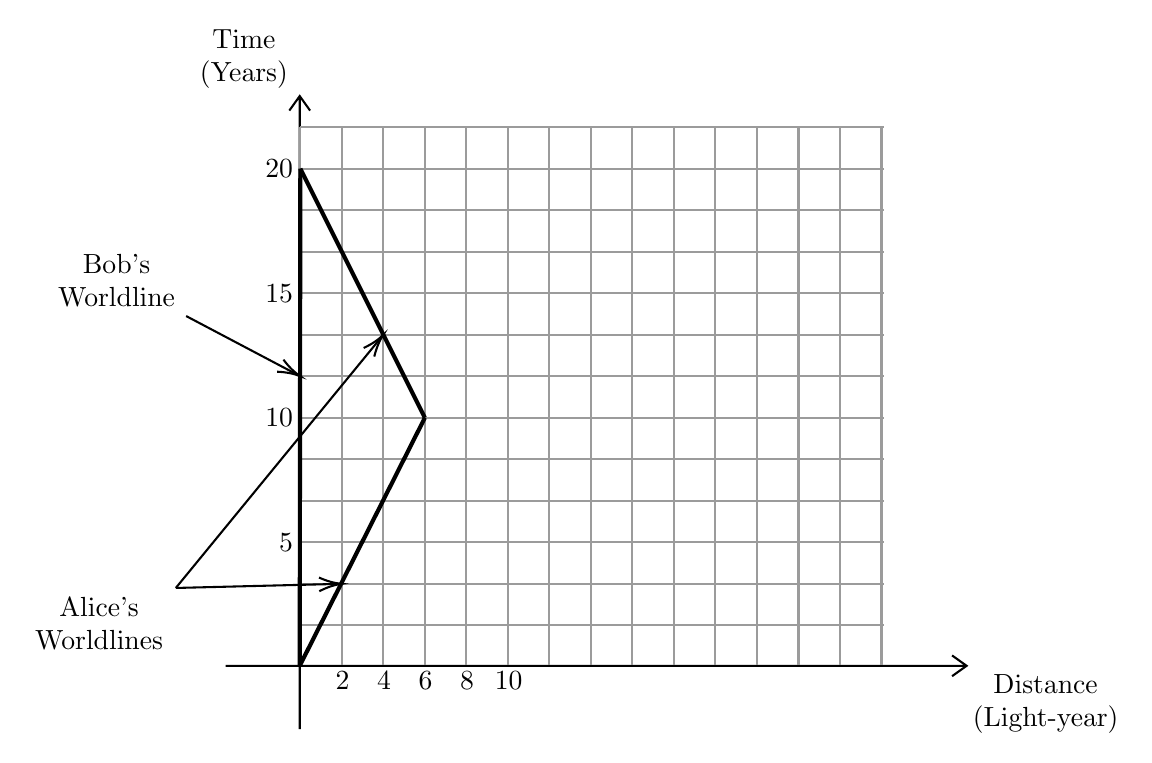
\begin{tikzpicture}[x=0.75pt,y=0.75pt,yscale=-1,xscale=1]
%uncomment if require: \path (0,420); %set diagram left start at 0, and has height of 420

%Shape: Axis 2D [id:dp05573369305563469] 
\draw  (164,323.5) -- (521,323.5)(199.7,49) -- (199.7,354) (514,318.5) -- (521,323.5) -- (514,328.5) (194.7,56) -- (199.7,49) -- (204.7,56)  ;
%Shape: Grid [id:dp24983811424563274] 
\draw  [draw opacity=0] (200,64) -- (481,64) -- (481,323) -- (200,323) -- cycle ; \draw  [color={rgb, 255:red, 155; green, 155; blue, 155 }  ,draw opacity=1 ] (200,64) -- (200,323)(220,64) -- (220,323)(240,64) -- (240,323)(260,64) -- (260,323)(280,64) -- (280,323)(300,64) -- (300,323)(320,64) -- (320,323)(340,64) -- (340,323)(360,64) -- (360,323)(380,64) -- (380,323)(400,64) -- (400,323)(420,64) -- (420,323)(440,64) -- (440,323)(460,64) -- (460,323)(480,64) -- (480,323) ; \draw  [color={rgb, 255:red, 155; green, 155; blue, 155 }  ,draw opacity=1 ] (200,64) -- (481,64)(200,84) -- (481,84)(200,104) -- (481,104)(200,124) -- (481,124)(200,144) -- (481,144)(200,164) -- (481,164)(200,184) -- (481,184)(200,204) -- (481,204)(200,224) -- (481,224)(200,244) -- (481,244)(200,264) -- (481,264)(200,284) -- (481,284)(200,304) -- (481,304) ; \draw  [color={rgb, 255:red, 155; green, 155; blue, 155 }  ,draw opacity=1 ]  ;
%Straight Lines [id:da8614004001055997] 
\draw [line width=1.5]    (199.7,323.5) -- (260,204) ;
%Straight Lines [id:da31958266480703523] 
\draw [line width=1.5]    (200,84) -- (260,204) ;
%Straight Lines [id:da118241818687711] 
\draw [line width=1.5]    (200,84) -- (199.7,323.5) ;
%Straight Lines [id:da8500340120601242] 
\draw    (145,155) -- (198.23,183.07) ;
\draw [shift={(200,184)}, rotate = 207.8] [color={rgb, 255:red, 0; green, 0; blue, 0 }  ][line width=0.75]    (10.93,-3.29) .. controls (6.95,-1.4) and (3.31,-0.3) .. (0,0) .. controls (3.31,0.3) and (6.95,1.4) .. (10.93,3.29)   ;
%Straight Lines [id:da8248865101372049] 
\draw    (140,286) -- (238.73,165.55) ;
\draw [shift={(240,164)}, rotate = 129.34] [color={rgb, 255:red, 0; green, 0; blue, 0 }  ][line width=0.75]    (10.93,-3.29) .. controls (6.95,-1.4) and (3.31,-0.3) .. (0,0) .. controls (3.31,0.3) and (6.95,1.4) .. (10.93,3.29)   ;
%Straight Lines [id:da5391136210716794] 
\draw    (140,286) -- (218,284.05) ;
\draw [shift={(220,284)}, rotate = 178.57] [color={rgb, 255:red, 0; green, 0; blue, 0 }  ][line width=0.75]    (10.93,-3.29) .. controls (6.95,-1.4) and (3.31,-0.3) .. (0,0) .. controls (3.31,0.3) and (6.95,1.4) .. (10.93,3.29)   ;

% Text Node
\draw (197.81,47) node [anchor=south east] [inner sep=0.75pt]   [align=left] {\begin{minipage}[lt]{35.23pt}\setlength\topsep{0pt}
\begin{center}
Time\\(Years)
\end{center}

\end{minipage}};
% Text Node
\draw (521,326) node [anchor=north west][inner sep=0.75pt]   [align=left] {\begin{minipage}[lt]{54.88pt}\setlength\topsep{0pt}
\begin{center}
Distance\\(Light-year)
\end{center}

\end{minipage}};
% Text Node
\draw (198,264) node [anchor=east] [inner sep=0.75pt]   [align=left] {5};
% Text Node
\draw (198,204) node [anchor=east] [inner sep=0.75pt]   [align=left] {10};
% Text Node
\draw (198,144) node [anchor=east] [inner sep=0.75pt]   [align=left] {15};
% Text Node
\draw (198,84) node [anchor=east] [inner sep=0.75pt]   [align=left] {20};
% Text Node
\draw (220.38,325) node [anchor=north] [inner sep=0.75pt]   [align=left] {2};
% Text Node
\draw (240.38,325) node [anchor=north] [inner sep=0.75pt]   [align=left] {4};
% Text Node
\draw (260.38,325) node [anchor=north] [inner sep=0.75pt]   [align=left] {6};
% Text Node
\draw (280.38,325) node [anchor=north] [inner sep=0.75pt]   [align=left] {8};
% Text Node
\draw (300.38,325) node [anchor=north] [inner sep=0.75pt]   [align=left] {10};
% Text Node
\draw (143,152) node [anchor=south east] [inner sep=0.75pt]   [align=left] {\begin{minipage}[lt]{45.05pt}\setlength\topsep{0pt}
\begin{center}
Bob's\\Worldline
\end{center}

\end{minipage}};
% Text Node
\draw (138,289) node [anchor=north east] [inner sep=0.75pt]   [align=left] {\begin{minipage}[lt]{50.15pt}\setlength\topsep{0pt}
\begin{center}
Alice's\\Worldlines
\end{center}

\end{minipage}};


\end{tikzpicture}
